\documentclass[11pt,a4paper,parskip=half ]{scrartcl}
\usepackage[utf8]{inputenc}
\usepackage[ngerman]{babel}
\usepackage{amsmath}
\usepackage{amsfonts}
\usepackage{amssymb}
\usepackage{graphicx}
\usepackage{xcolor}
\author{Aaron Winziers - 1176638}
\title{Informationsvisualisierung SS 2019\\\LARGE{Übungsblatt 1}}

\begin{document}
	\maketitle
	
	\section*{Aufgabe 1}
	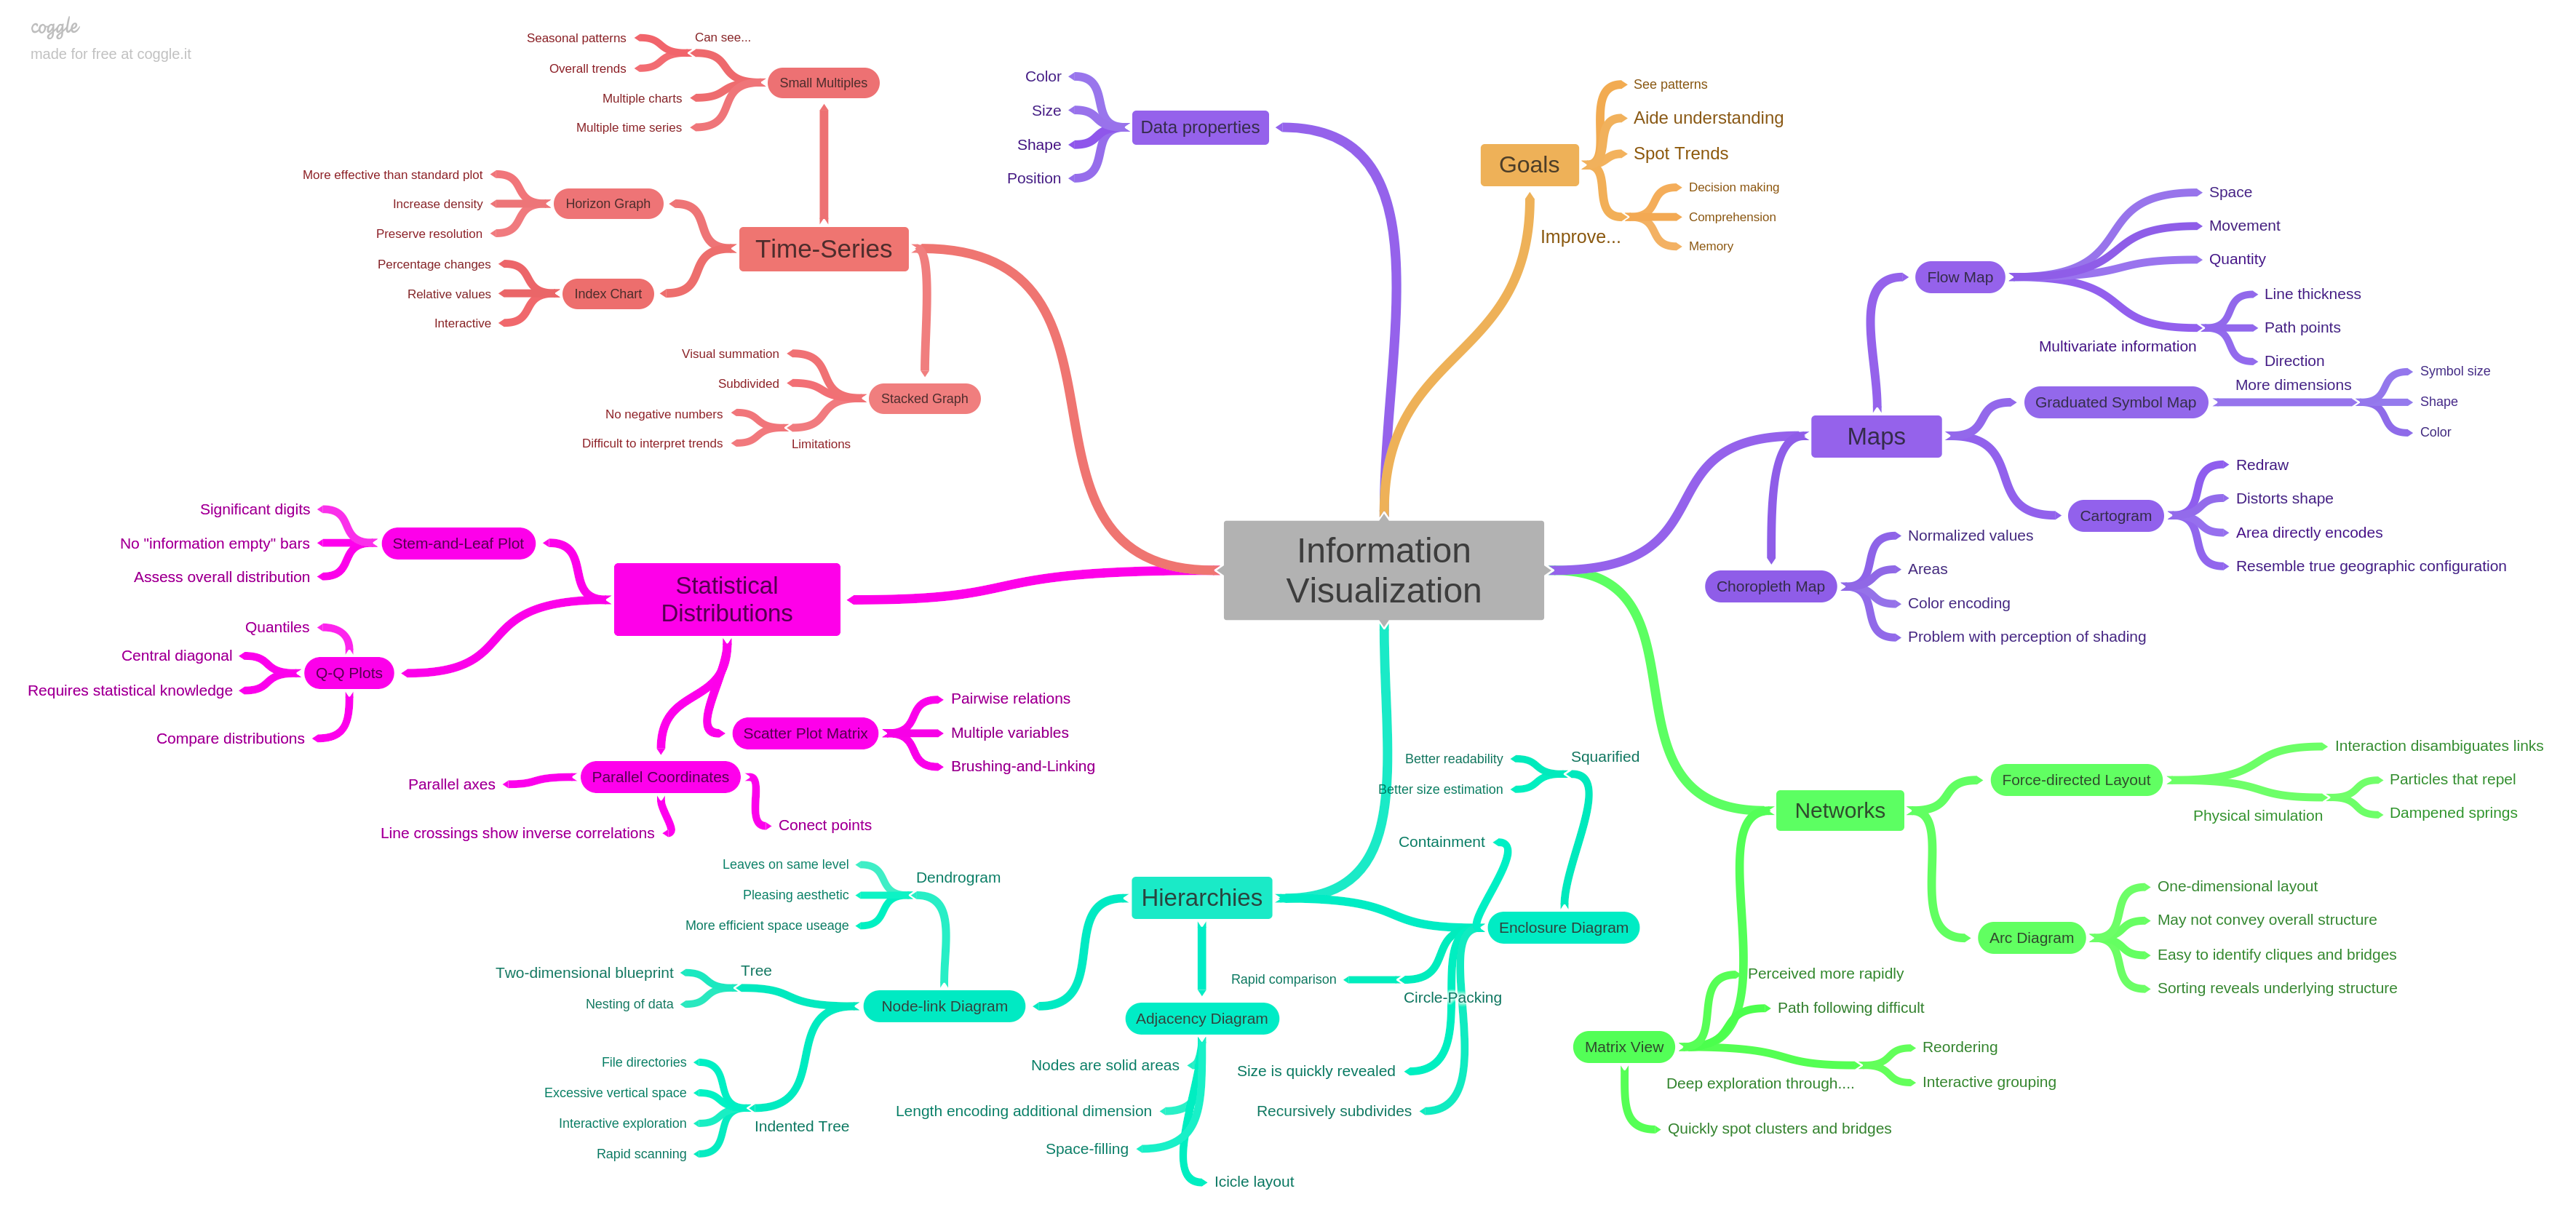
\includegraphics[width=\textwidth]{infvis_mindmap.png}
	
	
	\newpage
	Aaron Winziers - 1176638
	\section*{Aufgabe 2}
	\begin{table}[h]
		\begin{tabular}{p{2.5cm}||p{2.5cm}|p{2.5cm}|p{2.5cm}|p{2.5cm}}
			& Position                                                 & Size                                                                                     & Shape                       & Color                                                      \\ \hline \hline
			Parallel coordinates & Postion of dimensions can reveal different relationships & Plays no role                                                                            & Plays no role               & Allows for better readability                              \\ \hline
			Choropleth           & Shows the geographic layout                              & Shows the geographic layout, and must be taken into account as values must be normalized & Shows the geographic layout & Maps data to the regions in the map                        \\ \hline
			Treemap layout       & Child nodes are placed within parent nodes               & Represents the size of the classes the nodes represent                                   & Square quickly reveals size & Can be used to distinguish between parent nodes and leaves \\ \hline
			Matrix View          & May reveal clusters and bridges                          & Is dependent on the number of nodes                                                      & Plays no role               & Maps data to the                                          
		\end{tabular}
	\end{table}
	
\end{document}